\appendix
\chapter{Appendix}
 \label{appendix}
\section{Auxiliary Information}
 \label{aux_info}

\subsection{Text Indices \& FM-Index}
\label{fmindex}

\Glspl{text index} (also called \textit{substring indices} or \textit{full-text indices}) are data structures specifically meant for finding substrings within a \gls{text} in sub-linear time. They are explained in detail in a referenced survey paper~\cite{fmfordummies}. As the initialization of the text is costly, text indices are only worthwhile when numerous \glspl{query} for substrings of the same text are expected. Text indices work by traversing the contents of the given text and making annotations or restructuring them as necessary to `front-load' the work that queries would need to do; This can be thought of as `constructing a text index around a text'.
 
The FM-Index primarily uses a Burrows-Wheeler-Transformed text string as well as as \textit{suffix index} to store the relevant information. The details of Burrows-Wheeler Transform are briefly summarized in \ref{bwt}. Intuitively, the transformed text encodes which symbols \textit{precede} one another within the original text string. Due to its structure, all \glspl{match location} for a query are always `represented' by adjacent symbols in this \textsc{bwt}-string, allowing the full set of match locations to be stored in just two numbers: the bounds of a range. The index incrementally matches to a \gls{query} from back to front by essentially \textit{specifying} the matched substring, updating the match set range accordingly; At each step, the range represents the occurrences of the suffix of the query already matched. Each step of the matching process calls a subroutine often called `rank' or `occurrences', necessary for finding the range of the next node in the index search tree. The cost of this rank call varies depending on source; Often it is given as a \textit{large constant}.
 
The nature of the \textsc{bwt} facilitates \textit{backwards search}, specifying the query string from back to front. Many relevant procedures involving this search conceptually reason using a \textit{forwards search}, which differs only in the order of traversal. The iterative steps of this search are integrally-related to the partition \glspl{block} and \glspl{filter} used in the \aspop{} solution; These notions are usually described \textit{forwards} in the literature. A forwards search in the FM-Index can be simulated by initializing the text index on a \textit{reversed} text; These counter-intuitive representations are encapsulated inside the FM-Index and are not visible outside of it. For more details about how the implementation deals with this detail, see Section \ref{own_impl_search_dir}.


\subsection{Burrows-Wheeler Transform}
\label{bwt}

\textit{Burrows-Wheeler Transform} (or \textsc{bwt} for short) is a procedure that returns a permutation of some input string $s$ with specific desirable properties. The transformation can also be reverted if necessary. \textsc{bwt} strings tend to contain many \textit{runs} of the same symbols, allowing for some compression potential. Additionally, and more importantly for our purposes, the transformed string $s'$ is able to encode additional information about the sequence of characters in the original string without taking up any extra space.
 
For the procedure, $s$ is assumed to be end-delimited by an extra-alphabetic symbol, conventionally `\$'. The \textsc{bwt}-string is computed as follows:

\begin{enumerate}
\item For all rotations of $s$, create a row in a matrix, where a \textit{rotation} is $s[i+1,|s|]s[1,i]$ for $1\leq{} i \leq{|s|}$.
\item Sort the rows of the matrix according to a left-to-right lexicographic ordering of their symbols.
\item Return $s'$, the string represented by the symbols in the last column of the matrix, read from top to bottom.
\end{enumerate}

Ultimately, only $s'$ is retained, with the rest of the matrix and other intermediate data discarded. As $s$ and $s'$ are composed of columns from this same matrix, clearly $|s|=|s'|$.

If necessary, the first column of the matrix can be reacquired by simply sorting the symbols in $s'$. Then $s$ can be reconstructed from back to front beginning with the terminal `\$', with all preceding symbols `looked up' using the first and last columns of the \textsc{bw}-matrix.



% \section{Experiment Raw Data}

% \subsection{Phase 1}

% \begin{sidewaystable}[!htbp]
%     \centering
%     \caption{Phase 1 false negative counts of \aspop{} solver runs across multiple values of \bfit{t} and \bfit{e}. True solution set contains 4854458 elements.}
%     \label{table:phase1neg}
% \csvautobooktabular{data/negs_trans_labels.csv}
% \end{sidewaystable}

% \begin{sidewaystable}[!htbp]
%     \centering
%     \caption{Phase 1 false positive counts of \aspop{} solver runs across multiple values of \bfit{t} and \bfit{e}.}
%     \label{table:phase1pos}
% \csvautobooktabular{data/poss_trans_labels.csv}
% \end{sidewaystable}

\newpage
\section{Thesis Task Breakdown}

\begin{figure}[!htb]
\centering
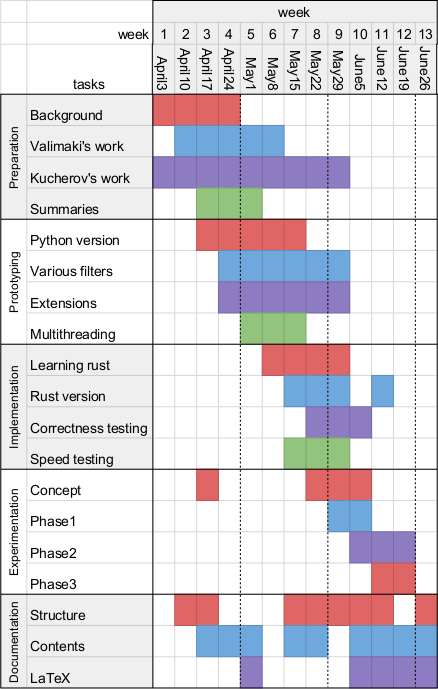
\includegraphics[width=0.7\textwidth]{images/sheet.png}
\caption{Thesis task breakdown per week.}
\label{fig:planner}
\end{figure}
